%%%%%%%%%%%%%%%%%%%%%%%%%%%%%%%%%%%%%%%%%%%%%%%%%%%%%%%%%%%%%%%%%%%%%%%%%%%%%%
% Nature-Style Template: FEM Simulation of Waveguide Eigenmodes
%%%%%%%%%%%%%%%%%%%%%%%%%%%%%%%%%%%%%%%%%%%%%%%%%%%%%%%%%%%%%%%%%%%%%%%%%%%%%%
\documentclass[10pt,letterpaper]{article}
\usepackage{times}
\usepackage{graphicx}
\usepackage{amsmath, amssymb}
\usepackage{color}
\usepackage{authblk}
\usepackage{caption}
\usepackage{subcaption}
\usepackage{geometry}
\geometry{margin=1in}
\usepackage{setspace}
\onehalfspacing

% Title, authors and affiliations
\title{\bf Finite Element Method for Eigenmode Analysis of Waveguides}
\author[1]{Yushi Zhou}
\affil[1]{Department of Electrical and Computer Engineering}
\date{}

\begin{document}
\maketitle
\thispagestyle{empty}

%%%%%%%%%%%%%%%%%%%%%%%%%%%%%%%%%%%%%%%%%%%%%%%%%%%%%%%%%%%%%%%%%%%%%%%%%%%%%%
\begin{abstract}
A finite element method (FEM) approach is presented for solving the 
eigenmode problem for waveguide structures. In particular, 
the formulation and implementation of the FEM methodology
 for eigenmode analysis is described, including mesh generation, matrix assembly, 
 and subsequent eigenvalue solution. Analytical results for a metallic 
 waveguide are developed for comparison. In addition, FEM simulations of
  a silicon waveguide embedded in air with perfectly matched layer (PML) 
  boundaries are analyzed. 
\end{abstract}

%%%%%%%%%%%%%%%%%%%%%%%%%%%%%%%%%%%%%%%%%%%%%%%%%%%%%%%%%%%%%%%%%%%%%%%%%%%%%%
\section*{Introduction}
Waveguide devices are critical components for photonic and communication systems.
 Accurate eigenmode analysis is essential for characterizing propagation 
 properties. Finite element methods provide a flexible numerical framework
 that accommodates complex geometries and material inhomogeneities. 
 In this work, we detail an FEM approach for solving the eigenmode 
 problem in rectangular waveguides. We first introduce the FEM methodology 
 and then present an analytical solution for the metallic waveguide case. 
 Then, we apply FEM implementation to a both a metallic waveguide and
 a silicon waveguide in air 
 with a PML boundary condition.

%%%%%%%%%%%%%%%%%%%%%%%%%%%%%%%%%%%%%%%%%%%%%%%%%%%%%%%%%%%%%%%%%%%%%%%%%%%%%%
\section*{Methods}
\subsection*{FEM Methodology}
Consider a partial differential eqution give by 
\begin{equation}
\mathcal{L} \varphi = f
\end{equation}
We can expand the solution $\varphi$ in terms of a set of basis functions $\varphi = \sum_{j=1}^{N} c_j \psi_j$
where $c_j$ are the coefficients to be determined. The weak form of the equation 
is obtained by multiplying by a test function $\psi_i$ and integrating over the 
domain $\Omega${\cite{jin2015theory}}: 
\begin{equation}
\int_{\Omega} w_i \mathcal{L} \left( \sum_{j=1}^{N} c_j \psi_j \right) \, \mathrm{d}\Omega = \int_{\Omega} w_i f \, \mathrm{d}\Omega
\end{equation}
In Galerkin's method, we choose the test function to be the same as the basis function,
\begin{equation}
\sum_{j=1}^{N} S_{ij} c_j = b_i \quad i = 1, 2, \ldots, N 
\end{equation}
where 
\begin{equation}
S_{ij} \equiv \int_{\Omega} v_i \left( \mathcal{L} \psi_j \right) \, \mathrm{d}\Omega 
\end{equation}
and 
\begin{equation}
b_i \equiv \int_{\Omega} v_i f \, \mathrm{d}\Omega 
\end{equation}

Specifically, for waveguide TE modes, the wave equation is given by
\begin{equation}
\left( \nabla^2 + k_c^2 \right) \mathbf{H}_z = 0
\end{equation}
Where $k_c$ is the cutoff wavenumber. Metallic waveguides have the boundary condition
\begin{equation}
\mathbf{n} \times \mathbf{H} = 0
\end{equation}

This corresponds to zero tangential magnetic field at the metallic walls. This boundary condition gives rise to the eigenvalue problem we solve.

Starting from the wave equation and applying the Galerkin method with test functions $N_i$:
\begin{equation}
\iint_\Omega N_i(\nabla^2 + k_c^2)H_z \, \mathrm{d}\Omega = 0
\end{equation}

Applying integration by parts (Green's first identity) to the Laplacian term:
\begin{equation}
\iint_\Omega N_i \nabla^2 H_z \, \mathrm{d}\Omega = -\iint_\Omega \nabla N_i \cdot \nabla H_z \, \mathrm{d}\Omega + \oint_{\partial\Omega} N_i \frac{\partial H_z}{\partial n} \, \mathrm{d}S
\end{equation}

Due to the boundary conditions, the boundary integral vanishes. Expanding $H_z \approx \sum_{j=1}^{N} H_j N_j$ and substituting:
\begin{align}
-\iint_\Omega \nabla N_i \cdot \nabla \left(\sum_{j=1}^{N} H_j N_j\right) \, \mathrm{d}\Omega + k_c^2 \iint_\Omega N_i \left(\sum_{j=1}^{N} H_j N_j\right) \, \mathrm{d}\Omega = 0
\end{align}

After simplification, we arrive at the generalized eigenvalue problem:
\begin{equation}
[A](H_z) = k_c^2 [B](H_z)
\end{equation}

Where the matrices $A$ and $B$ represent the discretized forms of the differential operator and are given by:
\begin{align*}
A_{ij} &= \iint_{\Omega} \nabla N_i \cdot \nabla N_j \, \mathrm{d}\Omega \qquad i,j=1,2,\dots,N \\
B_{ij} &= \iint_{\Omega} N_i N_j \, \mathrm{d}\Omega \qquad i,j=1,2,\dots,N
\end{align*}

Here, $N_i$ and $N_j$ are the interpolation functions defined for each element, 
and the integrals are computed over the entire problem domain $\Omega$. 
The matrix $A$ corresponds to the stiffness matrix, while $B$ corresponds to
 the mass matrix in the FEM formulation. The eigenvalues $k_c^2$ represent the squared cutoff wavenumbers of the waveguide modes.

\paragraph{Mesh Building and Basis functions:}  
In this problem, we use triangular elements to discretize the waveguide domain. 
The mesh is generated using MATLAB's PDE-toolbox function. Linear basis functions
are used for the triangular elements, which are defined as
\begin{equation}
\phi_i(x,y) = a_i + b_i x + c_i y
\end{equation}
where the coefficients $a_i$, $b_i$, and $c_i$ are determined by the nodal coordinates. These linear basis functions have the property that they equal 1 at their corresponding node and 0 at all other nodes. The gradients of these basis functions are constants within each element.
The generated mesh for the metallic waveguide model is shown in Fig. \ref{fig:mesh}, which illustrates a 33 × 14 mm rectangular domain discretized with triangular elements. 
\begin{figure}[htbp]
    \centering
    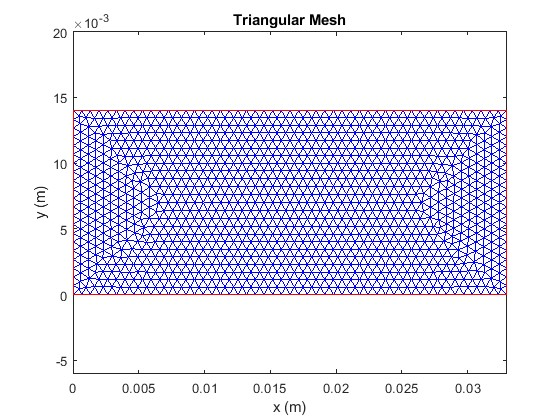
\includegraphics[width=0.8\linewidth]{mesh1.jpg}
    \caption{Triangular mesh generated for a 33 × 14 mm metallic waveguide with maximum element size of 33/50 mm.}
    \label{fig:mesh}
\end{figure}

\paragraph{Matrix Assembly:}  
The FEM algorithm builds the global matrices by assembling contributions from individual elements. For each triangular element, we first identify the element nodes and extract their coordinates. Then, we calculate the element area and the gradients of the basis functions within that element.

For triangular elements with nodes $i$, $j$, and $k$, the gradients of the linear basis functions are given by:
\begin{align}
\nabla \phi_i &= \frac{1}{2A_e}[y_j - y_k, x_k - x_j]^{T} \\
\nabla \phi_j &= \frac{1}{2A_e}[y_k - y_i, x_i - x_k]^{T} \\
\nabla \phi_k &= \frac{1}{2A_e}[y_i - y_j, x_j - x_i]^{T}
\end{align}

where $A_e$ is the area of the triangular element calculated as:
\begin{equation}
A_e = \frac{1}{2}|(x_j-x_i)(y_k-y_i) - (x_k-x_i)(y_j-y_i)|
\end{equation}

The element stiffness matrix $K_e$ is calculated using the dot products of these gradients:
\begin{equation}
K_{e,mn} = \iint_{\Omega_e} \nabla \phi_m \cdot \nabla \phi_n \, \mathrm{d}\Omega = \frac{1}{4A_e} (\mathbf{b}_m \cdot \mathbf{b}_n)
\end{equation}

where $\mathbf{b}_m = [y_j - y_k, x_k - x_j]^{T}$ for $m=i$ (and similar expressions for $j$ and $k$).

For the mass matrix, we use the standard formula for linear triangular elements:
\begin{equation}
M_{e,mn} = \iint_{\Omega_e} \phi_m \phi_n \, \mathrm{d}\Omega = \frac{A_e}{12}
\begin{cases}
2, & \text{if } m = n \\
1, & \text{if } m \neq n
\end{cases}
\end{equation}

The global matrices are assembled by adding each element's contribution to the appropriate positions determined by the element's nodal connectivity:
\begin{equation}
K_{IJ} = \sum_{e \in \Omega} K^e_{ij} \quad \text{and} \quad M_{IJ} = \sum_{e \in \Omega} M^e_{ij}
\end{equation}

where $I$ and $J$ are the global indices of nodes $i$ and $j$ in element $e$.

\paragraph{Theoretical solution for metallic waveguide:}  
For a rectangular metallic waveguide with dimensions $a \times b$ (width $\times$ height), the TE modes have well-established analytical solutions. The magnetic field in the $z$-direction for the TE$_{mn}$ mode can be expressed as:
\begin{equation}
H_z(x,y) = H_0 \cos\left(\frac{m\pi x}{a}\right) \cos\left(\frac{n\pi y}{b}\right)
\end{equation}
where $m$ and $n$ are non-negative integers that cannot be simultaneously zero. The corresponding cutoff wavenumber for each TE$_{mn}$ mode is given by:
\begin{equation}
k_{c,mn} = \sqrt{\left(\frac{m\pi}{a}\right)^2 + \left(\frac{n\pi}{b}\right)^2}
\end{equation}
From this cutoff wavenumber, we can calculate the cutoff frequency:
\begin{equation}
f_{c,mn} = \frac{c}{2\pi}k_{c,mn} = \frac{c}{2}\sqrt{\left(\frac{m}{a}\right)^2 + \left(\frac{n}{b}\right)^2}
\end{equation}
where $c$ is the speed of light in vacuum. 
\paragraph{Theoretical Mode Patterns:}
For the first few TE modes in a rectangular waveguide, the field patterns can be characterized by their indices $(m,n)$. The dominant mode is usually TE$_{10}$ (where $m=1, n=0$), which has the lowest cutoff frequency. As the mode indices increase, the field patterns become more complex with additional variations along the width and height dimensions.

For a waveguide with dimensions $a \times b$ where $a > b$, the first 9 TE modes in order of increasing cutoff frequency are typically: TE$_{10}$, TE$_{20}$, TE$_{01}$, TE$_{11}$, TE$_{21}$, TE$_{30}$, TE$_{31}$, TE$_{40}$, and TE$_{02}$ (though the exact ordering depends on the aspect ratio of the waveguide).

Each mode exhibits a distinct field pattern characterized by $m$ half-sinusoidal variations along the $x$-direction and $n$ half-sinusoidal variations along the $y$-direction. The mode distributions thus form standing wave patterns within the cross-section of the waveguide.

\begin{figure}[htbp]
    \centering
    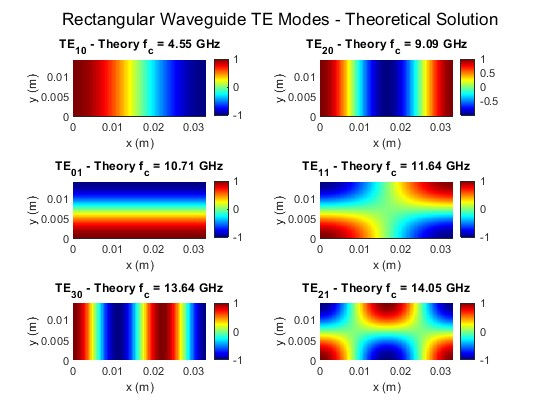
\includegraphics[width=0.8\linewidth]{2.jpg}
    \caption{Theoretical Hz distributions for the first six TE modes in a rectangular metallic waveguide, showing the characteristic standing wave patterns based on analytical expressions.}
    \label{fig:theory_modes}
\end{figure}

%%%%%%%%%%%%%%%%%%%%%%%%%%%%%%%%%%%%%%%%%%%%%%%%%%%%%%%%%%%%%%%%%%%%%%%%%%%%%%
\section*{Results}
\subsection*{Part 1: Metallic Waveguide}
The FEM simulation was conducted for a rectangular metallic 
waveguide using the methodology described above. Figure 
\ref{fig:mode_patterns} shows the Hz field distributions 
for the first six eigenmodes computed using a fine mesh 
(maximum element size of Length/200).

\begin{figure}[htbp]
    \centering
    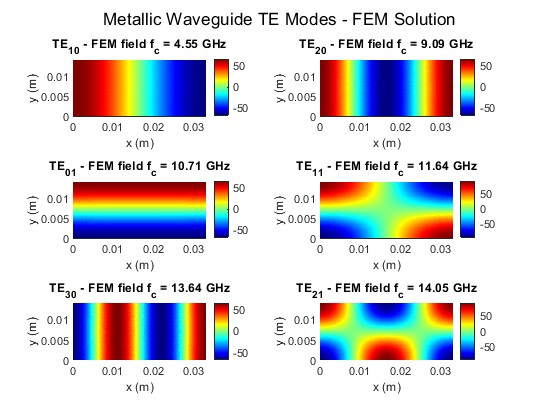
\includegraphics[width=0.8\linewidth]{1.jpg}
    \caption{FEM simulation results showing Hz distributions for the first six TE modes in the rectangular metallic waveguide using a fine mesh with extra fine mesh.}
    \label{fig:mode_patterns}
\end{figure}

\paragraph{Mode Analysis Results:}
Table \ref{tab:cutoff_freq} presents the computed cutoff wavenumbers and corresponding frequencies for the first six modes using the fine mesh.

\begin{table}[htbp]
    \centering
    \caption{Computed cutoff wavenumbers and frequencies for the first six modes}
    \begin{tabular}{ccc}
    \hline
    Mode & Cutoff k (rad/m) & Cutoff f (GHz) \\
    \hline
     1   &      95.20      &      4.55     \\
     2   &     190.41      &      9.09     \\
     3   &     224.41      &     10.71     \\
     4   &     243.77      &     11.64     \\
     5   &     285.62      &     13.64     \\
     6   &     294.31      &     14.05     \\
    \hline
    \end{tabular}
    \label{tab:cutoff_freq}
\end{table}

The simulation results show excellent agreement with theoretical values, with the average error for the six modes being only 0.0046\% when using the fine mesh. 

\paragraph{Convergence Analysis:}
To investigate the impact of mesh resolution on solution accuracy, a convergence study was performed using progressively coarser meshes. Table \ref{tab:convergence} summarizes the average percentage error in cutoff frequencies for different mesh resolutions.

\begin{table}[htbp]
    \centering
    \caption{Convergence study showing average error percentage for different mesh resolutions}
    \begin{tabular}{cc}
    \hline
    Mesh resolution (hmax) & Average error (\%) \\
    \hline
    Length/200 & 0.0046 \\
    Length/100 & 0.0186 \\
    Length/50  & 0.0754 \\
    Length/25  & 0.2117 \\
    Length/10  & 1.4051 \\
    \hline
    \end{tabular}
    \label{tab:convergence}
\end{table}

The convergence study demonstrates that even relatively coarse meshes can produce accurate results for waveguide eigenvalue problems. For instance, a mesh with maximum element size of Length/50 yields an average error of only 0.0754\%. This efficiency is particularly beneficial for computational performance, as the simulations executed rapidly even on a single-core CPU. Even for the finest mesh (Length/200), the computation completed in just a few seconds.


\subsection*{Part 2: Silicon Waveguide with Air and PML Boundary Condition}
For the silicon waveguide analysis, we extend our simulation to another scenario involving a dielectric waveguide surrounded by air with perfectly matched layer (PML) boundary conditions. 
\paragraph{Material Configuration:} 
The mesh building and basis function selection followed the same methodology as the metallic waveguide case. However, the material properties were assigned differently to account for the inhomogeneous structure. The waveguide consists of a silicon core (Si) with relative permittivity $\varepsilon_{Si} = 12.04$ surrounded by air with relative permittivity $\varepsilon_{air} = 1$.

Material properties were assigned to each element by examining the position of its centroid. For each triangular element, we calculated the centroid coordinates $(x_c, y_c)$ by averaging the coordinates of its three vertices:
\begin{equation}
x_c = \frac{x_i + x_j + x_k}{3}, \quad y_c = \frac{y_i + y_j + y_k}{3}
\end{equation}

Elements with centroids located within the silicon region (defined as $0 \leq x \leq a$ and $0 \leq y \leq b$, where $a$ and $b$ are the width and height of the silicon core) were assigned $\varepsilon_{Si}$, while all other elements were assigned $\varepsilon_{air}$. This material distribution was then incorporated into the FEM formulation, modifying the mass matrix to include the spatially varying permittivity:

\begin{equation}
B_{ij} = \iint_{\Omega} \varepsilon_r(x,y) N_i N_j \, \mathrm{d}\Omega
\end{equation}

\paragraph{PML Implementation:} 
To model the open boundary conditions required for the silicon waveguide, we implemented perfectly matched layers (PML) using the complex coordinate stretching technique. The PML creates an artificial absorbing region at the simulation domain boundaries that prevents reflections of outgoing electromagnetic waves.

The coordinate stretching is defined by complex scaling factors:
\begin{equation}
\tilde{x} = \int s_x(x') dx', \quad \tilde{y} = \int s_y(y') dy'
\end{equation}
where $s_x(x)$ and $s_y(y)$ are the complex stretching functions:
\begin{equation}
s_x(x) = 1 + i\frac{\sigma_x(x)}{k_0}, \quad s_y(y) = 1 + i\frac{\sigma_y(y)}{k_0}
\end{equation}

The absorption profile $\sigma$ increases gradually from zero at the PML interface to $\sigma_{max}$ at the domain boundary following a polynomial function:
\begin{equation}
\sigma(d) = \sigma_{max}\left(\frac{d}{d_{pml}}\right)^n
\end{equation}
where $d$ is the distance into the PML layer, $d_{pml}$ is the PML thickness, and $n$ is the polynomial order (typically 3).

This coordinate transformation modifies both the stiffness and mass matrices in the FEM formulation. The gradient operator is transformed according to the coordinate stretching, while the integration measure includes the determinant of the stretching tensor $s_x \cdot s_y$:

\begin{equation}
K_{ij} = \iint_{\Omega} \left(\frac{1}{s_x}\frac{\partial N_i}{\partial x}\frac{1}{s_x}\frac{\partial N_j}{\partial x} + \frac{1}{s_y}\frac{\partial N_i}{\partial y}\frac{1}{s_y}\frac{\partial N_j}{\partial y} \right) s_x s_y \, \mathrm{d}\Omega
\end{equation}

\begin{equation}
B_{ij} = \iint_{\Omega} \varepsilon_r(x,y) N_i N_j \, s_x s_y \, \mathrm{d}\Omega
\end{equation}

This formulation allows waves to propagate into the PML region where they decay exponentially without reflection, effectively simulating an infinite domain within our finite computational space.

\paragraph{Simulation Results:} 
\paragraph{Simulation Results:} 
For the silicon waveguide simulation, we used a mesh with maximum element size of Length/100, providing a good balance between accuracy and computational efficiency. Fig. \ref{fig:si_mesh} shows the generated mesh with the silicon core highlighted.

\begin{figure}[htbp]
    \centering
    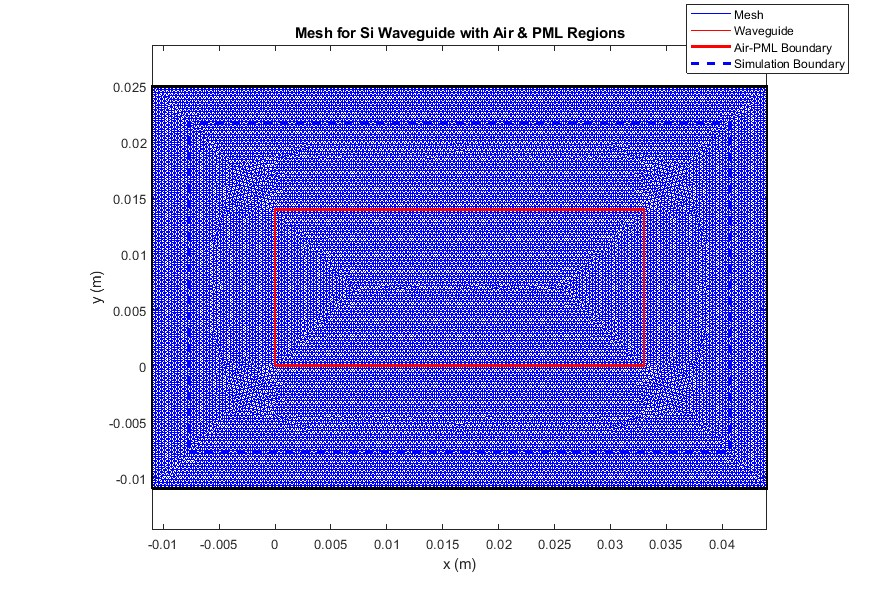
\includegraphics[width=0.8\linewidth]{4.jpg}
    \caption{Mesh generated for the silicon waveguide simulation, showing the silicon core region (highlighted) surrounded by air and PML boundary regions.}
    \label{fig:si_mesh}
\end{figure}

Table \ref{tab:si_results} presents the propagation constants ($\beta$) and effective refractive indices for the first six guided modes of the silicon waveguide.

\begin{table}[htbp]
    \centering
    \caption{Computed propagation constants and effective indices for the first six modes in the silicon waveguide}
    \begin{tabular}{ccc}
    \hline
    Mode & $\beta$ (rad/m) & Effective Index \\
    \hline
     1   &      35.02      &      0.0864     \\
     2   &      61.86      &      0.1526     \\
     3   &      63.02      &      0.1555     \\
     4   &      80.25      &      0.1980     \\
     5   &      85.35      &      0.2105     \\
     6   &      98.55      &      0.2431     \\
    \hline
    \end{tabular}
    \label{tab:si_results}
\end{table}

The effective index is defined as $n_{\text{eff}} = \beta/k_0$, 
where $\beta$ is the propagation constant and $k_0$ is 
the free-space wavenumber. Physically, 
it represents the ratio of the phase velocity of light in vacuum 
to the phase velocity of the guided mode. 
The effective index captures the combined effect of the waveguide
 geometry and materials on wave propagation. 
 The low effective index values in our results 
 show modes that are weakly confined with 
 much of their field extending into the air region.

Fig. \ref{fig:si_modes} shows the Hz field distributions for the first six eigenmodes of the silicon waveguide. Unlike the metallic waveguide case, these modes exhibit field patterns that extend beyond the core-cladding interface, with evanescent fields penetrating into the air region. The PML boundary condition effectively absorbs the outgoing waves without reflection, simulating an open boundary.

\begin{figure}[htbp]
    \centering
    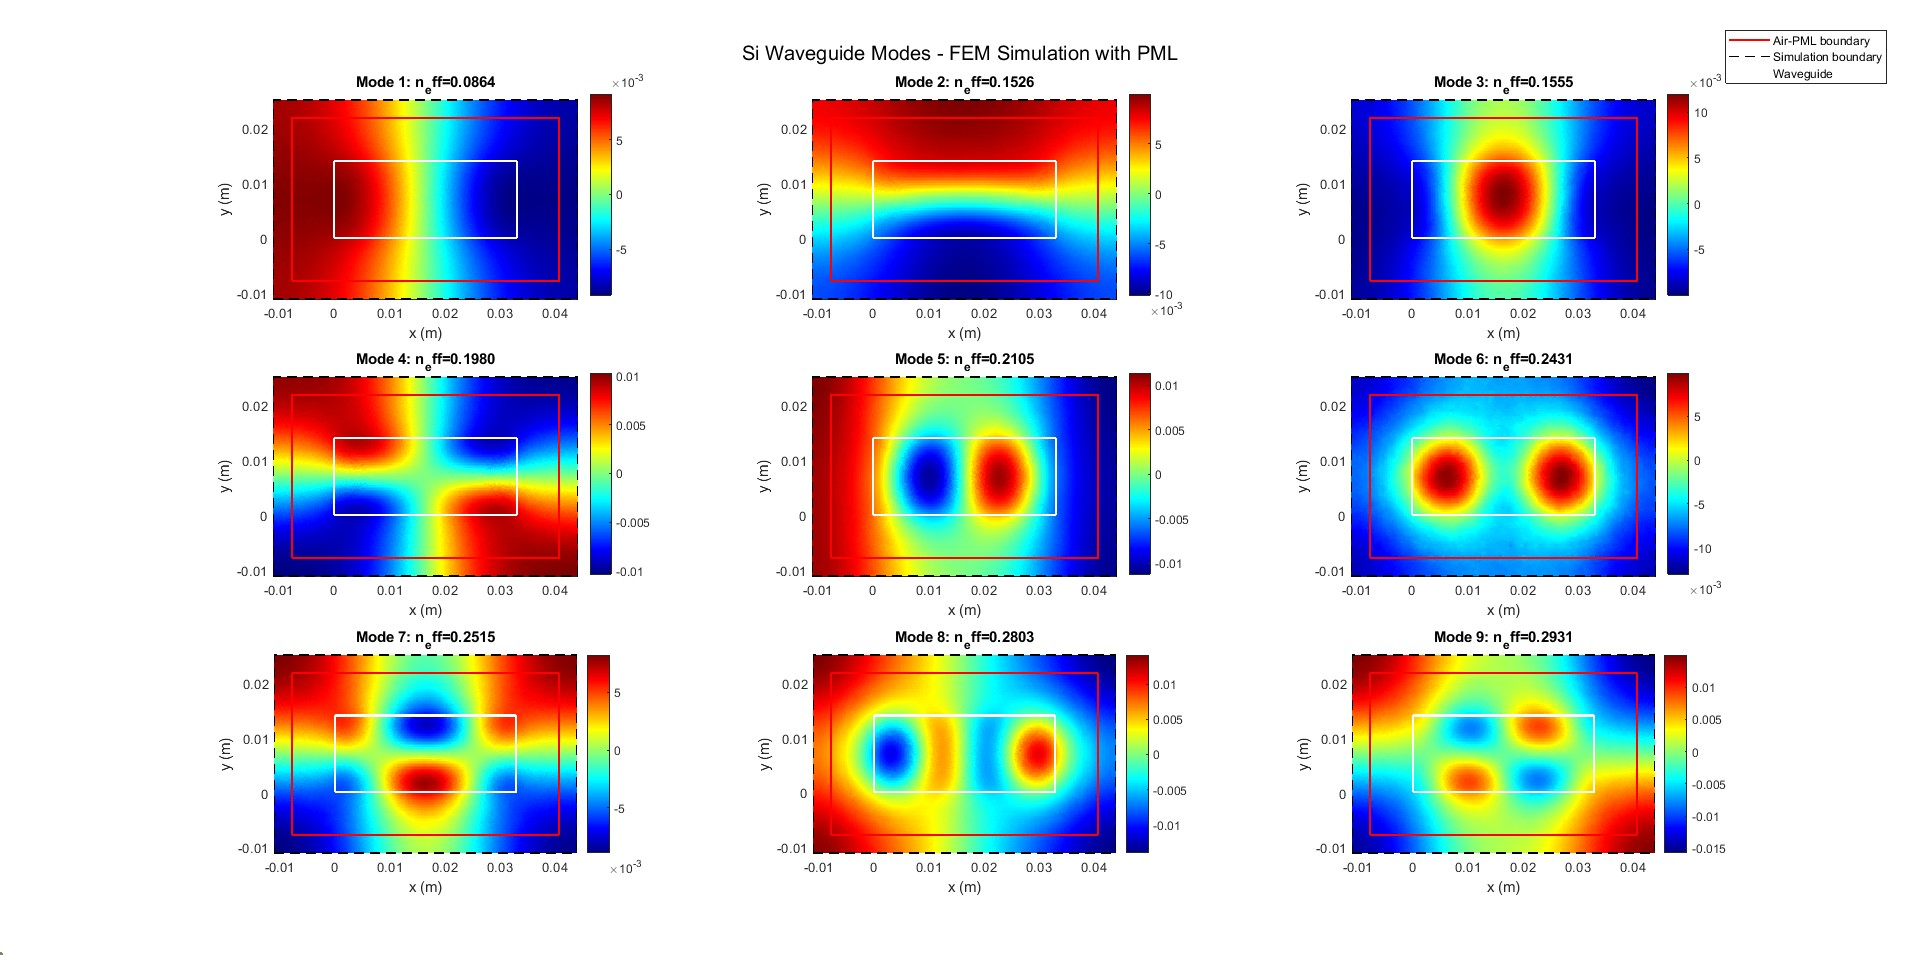
\includegraphics[width=1\linewidth]{3.jpg}
    \caption{FEM simulation results showing Hz distributions for the first six guided modes in the silicon waveguide. Note the field penetration into the air cladding and the effective absorption at the PML boundaries.}
    \label{fig:si_modes}
\end{figure}

%%%%%%%%%%%%%%%%%%%%%%%%%%%%%%%%%%%%%%%%%%%%%%%%%%%%%%%%%%%%%%%%%%%%%%%%%%%%%%
\section*{Conclusion}
In this study, we successfully implemented a finite element method (FEM) approach for eigenmode analysis of waveguides. The simulations of both metallic rectangular waveguide and silicon waveguide with PML boundary conditions demonstrated excellent accuracy. For the metallic waveguide, our FEM results converged rapidly with mesh refinement, 
achieving less than 0.01\% error using fine meshes. The silicon waveguide simulation effectively captured the guided modes with field extension into the air cladding. These results validate the robustness of our FEM implementation for waveguide eigenmode analysis and demonstrate its applicability to both metallic and dielectric waveguide structures.

%%%%%%%%%%%%%%%%%%%%%%%%%%%%%%%%%%%%%%%%%%%%%%%%%%%%%%%%%%%%%%%%%%%%%%%%%%%%%%

\begin{thebibliography}{9}
  \bibitem{jin2015theory} J.-M. Jin, \emph{Theory and Computation of Electromagnetic Fields}. Wiley, 2015.
\end{thebibliography}

%%%%%%%%%%%%%%%%%%%%%%%%%%%%%%%%%%%%%%%%%%%%%%%%%%%%%%%%%%%%%%%%%%%%%%%%%%%%%%
\end{document}
